%% ma: L12-B01-0003
%% lop: 12
%% chuong: 1
%% bai: 1
%% dang: 12.1.3
%% loai: TN4
%% muc: TH
%% dap_an: "B"
%% nguon: "(NBV)-ĐỀ SỐ 1-MỖI NGÀY 1 ĐỀ THI 2025.pdf (D01, MỖI NGÀY 1 ĐỀ - Đề số 1), Phần I Câu 1"
%% kien_thuc: "Bài 1 (tính đơn điệu của hàm số qua dấu của đạo hàm, bảng biến thiên)"
%% ghi_chu: "kho.py trung: 0,83 so với L12-B01-0002 chỉ vì cùng câu hỏi ngắn; khác nguồn dữ liệu (bảng biến thiên và đồ thị) nên không coi là trùng"
%% trang_thai: cho-duyet
%% ly_do: "Dạng mới đề xuất 12.1.3 (đọc khoảng đồng biến từ bảng biến thiên) chờ giáo viên duyệt"
\begin{ex}
Cho hàm số $f(x)$ có bảng biến thiên như sau:
\begin{center}
\begin{tikzpicture}
  \tkzTabInit[lgt=1.2,espcl=2.6]{$x$/.8,$f'(x)$/.8,$f(x)$/2}{$-\infty$,$-1$,$3$,$+\infty$}
  \tkzTabLine{,+,0,-,0,+,}
  \tkzTabVar{-/$-\infty$,+/$1$,-/$-3$,+/$+\infty$}
\end{tikzpicture}
\end{center}
Hàm số đã cho đồng biến trên khoảng nào sau đây?
\choice{$(-\infty;1)$}{\True $(3;+\infty)$}{$(-1;3)$}{$(-3;+\infty)$}
\loigiai{Từ bảng biến thiên, $f'(x)>0$ trên $(-\infty;-1)$ và $(3;+\infty)$ nên hàm số đồng biến trên các khoảng đó. Trong bốn phương án chỉ có $(3;+\infty)$ nằm trọn trong một khoảng đồng biến.}
\end{ex}
